% Options for packages loaded elsewhere
% Options for packages loaded elsewhere
\PassOptionsToPackage{unicode}{hyperref}
\PassOptionsToPackage{hyphens}{url}
\PassOptionsToPackage{dvipsnames,svgnames,x11names}{xcolor}
%
\documentclass[
  letterpaper,
  DIV=11,
  numbers=noendperiod]{scrreprt}
\usepackage{xcolor}
\usepackage{amsmath,amssymb}
\setcounter{secnumdepth}{5}
\usepackage{iftex}
\ifPDFTeX
  \usepackage[T1]{fontenc}
  \usepackage[utf8]{inputenc}
  \usepackage{textcomp} % provide euro and other symbols
\else % if luatex or xetex
  \usepackage{unicode-math} % this also loads fontspec
  \defaultfontfeatures{Scale=MatchLowercase}
  \defaultfontfeatures[\rmfamily]{Ligatures=TeX,Scale=1}
\fi
\usepackage{lmodern}
\ifPDFTeX\else
  % xetex/luatex font selection
\fi
% Use upquote if available, for straight quotes in verbatim environments
\IfFileExists{upquote.sty}{\usepackage{upquote}}{}
\IfFileExists{microtype.sty}{% use microtype if available
  \usepackage[]{microtype}
  \UseMicrotypeSet[protrusion]{basicmath} % disable protrusion for tt fonts
}{}
\makeatletter
\@ifundefined{KOMAClassName}{% if non-KOMA class
  \IfFileExists{parskip.sty}{%
    \usepackage{parskip}
  }{% else
    \setlength{\parindent}{0pt}
    \setlength{\parskip}{6pt plus 2pt minus 1pt}}
}{% if KOMA class
  \KOMAoptions{parskip=half}}
\makeatother
% Make \paragraph and \subparagraph free-standing
\makeatletter
\ifx\paragraph\undefined\else
  \let\oldparagraph\paragraph
  \renewcommand{\paragraph}{
    \@ifstar
      \xxxParagraphStar
      \xxxParagraphNoStar
  }
  \newcommand{\xxxParagraphStar}[1]{\oldparagraph*{#1}\mbox{}}
  \newcommand{\xxxParagraphNoStar}[1]{\oldparagraph{#1}\mbox{}}
\fi
\ifx\subparagraph\undefined\else
  \let\oldsubparagraph\subparagraph
  \renewcommand{\subparagraph}{
    \@ifstar
      \xxxSubParagraphStar
      \xxxSubParagraphNoStar
  }
  \newcommand{\xxxSubParagraphStar}[1]{\oldsubparagraph*{#1}\mbox{}}
  \newcommand{\xxxSubParagraphNoStar}[1]{\oldsubparagraph{#1}\mbox{}}
\fi
\makeatother

\usepackage{color}
\usepackage{fancyvrb}
\newcommand{\VerbBar}{|}
\newcommand{\VERB}{\Verb[commandchars=\\\{\}]}
\DefineVerbatimEnvironment{Highlighting}{Verbatim}{commandchars=\\\{\}}
% Add ',fontsize=\small' for more characters per line
\usepackage{framed}
\definecolor{shadecolor}{RGB}{241,243,245}
\newenvironment{Shaded}{\begin{snugshade}}{\end{snugshade}}
\newcommand{\AlertTok}[1]{\textcolor[rgb]{0.68,0.00,0.00}{#1}}
\newcommand{\AnnotationTok}[1]{\textcolor[rgb]{0.37,0.37,0.37}{#1}}
\newcommand{\AttributeTok}[1]{\textcolor[rgb]{0.40,0.45,0.13}{#1}}
\newcommand{\BaseNTok}[1]{\textcolor[rgb]{0.68,0.00,0.00}{#1}}
\newcommand{\BuiltInTok}[1]{\textcolor[rgb]{0.00,0.23,0.31}{#1}}
\newcommand{\CharTok}[1]{\textcolor[rgb]{0.13,0.47,0.30}{#1}}
\newcommand{\CommentTok}[1]{\textcolor[rgb]{0.37,0.37,0.37}{#1}}
\newcommand{\CommentVarTok}[1]{\textcolor[rgb]{0.37,0.37,0.37}{\textit{#1}}}
\newcommand{\ConstantTok}[1]{\textcolor[rgb]{0.56,0.35,0.01}{#1}}
\newcommand{\ControlFlowTok}[1]{\textcolor[rgb]{0.00,0.23,0.31}{\textbf{#1}}}
\newcommand{\DataTypeTok}[1]{\textcolor[rgb]{0.68,0.00,0.00}{#1}}
\newcommand{\DecValTok}[1]{\textcolor[rgb]{0.68,0.00,0.00}{#1}}
\newcommand{\DocumentationTok}[1]{\textcolor[rgb]{0.37,0.37,0.37}{\textit{#1}}}
\newcommand{\ErrorTok}[1]{\textcolor[rgb]{0.68,0.00,0.00}{#1}}
\newcommand{\ExtensionTok}[1]{\textcolor[rgb]{0.00,0.23,0.31}{#1}}
\newcommand{\FloatTok}[1]{\textcolor[rgb]{0.68,0.00,0.00}{#1}}
\newcommand{\FunctionTok}[1]{\textcolor[rgb]{0.28,0.35,0.67}{#1}}
\newcommand{\ImportTok}[1]{\textcolor[rgb]{0.00,0.46,0.62}{#1}}
\newcommand{\InformationTok}[1]{\textcolor[rgb]{0.37,0.37,0.37}{#1}}
\newcommand{\KeywordTok}[1]{\textcolor[rgb]{0.00,0.23,0.31}{\textbf{#1}}}
\newcommand{\NormalTok}[1]{\textcolor[rgb]{0.00,0.23,0.31}{#1}}
\newcommand{\OperatorTok}[1]{\textcolor[rgb]{0.37,0.37,0.37}{#1}}
\newcommand{\OtherTok}[1]{\textcolor[rgb]{0.00,0.23,0.31}{#1}}
\newcommand{\PreprocessorTok}[1]{\textcolor[rgb]{0.68,0.00,0.00}{#1}}
\newcommand{\RegionMarkerTok}[1]{\textcolor[rgb]{0.00,0.23,0.31}{#1}}
\newcommand{\SpecialCharTok}[1]{\textcolor[rgb]{0.37,0.37,0.37}{#1}}
\newcommand{\SpecialStringTok}[1]{\textcolor[rgb]{0.13,0.47,0.30}{#1}}
\newcommand{\StringTok}[1]{\textcolor[rgb]{0.13,0.47,0.30}{#1}}
\newcommand{\VariableTok}[1]{\textcolor[rgb]{0.07,0.07,0.07}{#1}}
\newcommand{\VerbatimStringTok}[1]{\textcolor[rgb]{0.13,0.47,0.30}{#1}}
\newcommand{\WarningTok}[1]{\textcolor[rgb]{0.37,0.37,0.37}{\textit{#1}}}

\usepackage{longtable,booktabs,array}
\usepackage{calc} % for calculating minipage widths
% Correct order of tables after \paragraph or \subparagraph
\usepackage{etoolbox}
\makeatletter
\patchcmd\longtable{\par}{\if@noskipsec\mbox{}\fi\par}{}{}
\makeatother
% Allow footnotes in longtable head/foot
\IfFileExists{footnotehyper.sty}{\usepackage{footnotehyper}}{\usepackage{footnote}}
\makesavenoteenv{longtable}
\usepackage{graphicx}
\makeatletter
\newsavebox\pandoc@box
\newcommand*\pandocbounded[1]{% scales image to fit in text height/width
  \sbox\pandoc@box{#1}%
  \Gscale@div\@tempa{\textheight}{\dimexpr\ht\pandoc@box+\dp\pandoc@box\relax}%
  \Gscale@div\@tempb{\linewidth}{\wd\pandoc@box}%
  \ifdim\@tempb\p@<\@tempa\p@\let\@tempa\@tempb\fi% select the smaller of both
  \ifdim\@tempa\p@<\p@\scalebox{\@tempa}{\usebox\pandoc@box}%
  \else\usebox{\pandoc@box}%
  \fi%
}
% Set default figure placement to htbp
\def\fps@figure{htbp}
\makeatother


% definitions for citeproc citations
\NewDocumentCommand\citeproctext{}{}
\NewDocumentCommand\citeproc{mm}{%
  \begingroup\def\citeproctext{#2}\cite{#1}\endgroup}
\makeatletter
 % allow citations to break across lines
 \let\@cite@ofmt\@firstofone
 % avoid brackets around text for \cite:
 \def\@biblabel#1{}
 \def\@cite#1#2{{#1\if@tempswa , #2\fi}}
\makeatother
\newlength{\cslhangindent}
\setlength{\cslhangindent}{1.5em}
\newlength{\csllabelwidth}
\setlength{\csllabelwidth}{3em}
\newenvironment{CSLReferences}[2] % #1 hanging-indent, #2 entry-spacing
 {\begin{list}{}{%
  \setlength{\itemindent}{0pt}
  \setlength{\leftmargin}{0pt}
  \setlength{\parsep}{0pt}
  % turn on hanging indent if param 1 is 1
  \ifodd #1
   \setlength{\leftmargin}{\cslhangindent}
   \setlength{\itemindent}{-1\cslhangindent}
  \fi
  % set entry spacing
  \setlength{\itemsep}{#2\baselineskip}}}
 {\end{list}}
\usepackage{calc}
\newcommand{\CSLBlock}[1]{\hfill\break\parbox[t]{\linewidth}{\strut\ignorespaces#1\strut}}
\newcommand{\CSLLeftMargin}[1]{\parbox[t]{\csllabelwidth}{\strut#1\strut}}
\newcommand{\CSLRightInline}[1]{\parbox[t]{\linewidth - \csllabelwidth}{\strut#1\strut}}
\newcommand{\CSLIndent}[1]{\hspace{\cslhangindent}#1}



\setlength{\emergencystretch}{3em} % prevent overfull lines

\providecommand{\tightlist}{%
  \setlength{\itemsep}{0pt}\setlength{\parskip}{0pt}}



 


\KOMAoption{captions}{tableheading}
\makeatletter
\@ifpackageloaded{tcolorbox}{}{\usepackage[skins,breakable]{tcolorbox}}
\@ifpackageloaded{fontawesome5}{}{\usepackage{fontawesome5}}
\definecolor{quarto-callout-color}{HTML}{909090}
\definecolor{quarto-callout-note-color}{HTML}{0758E5}
\definecolor{quarto-callout-important-color}{HTML}{CC1914}
\definecolor{quarto-callout-warning-color}{HTML}{EB9113}
\definecolor{quarto-callout-tip-color}{HTML}{00A047}
\definecolor{quarto-callout-caution-color}{HTML}{FC5300}
\definecolor{quarto-callout-color-frame}{HTML}{acacac}
\definecolor{quarto-callout-note-color-frame}{HTML}{4582ec}
\definecolor{quarto-callout-important-color-frame}{HTML}{d9534f}
\definecolor{quarto-callout-warning-color-frame}{HTML}{f0ad4e}
\definecolor{quarto-callout-tip-color-frame}{HTML}{02b875}
\definecolor{quarto-callout-caution-color-frame}{HTML}{fd7e14}
\makeatother
\makeatletter
\@ifpackageloaded{bookmark}{}{\usepackage{bookmark}}
\makeatother
\makeatletter
\@ifpackageloaded{caption}{}{\usepackage{caption}}
\AtBeginDocument{%
\ifdefined\contentsname
  \renewcommand*\contentsname{Table of contents}
\else
  \newcommand\contentsname{Table of contents}
\fi
\ifdefined\listfigurename
  \renewcommand*\listfigurename{List of Figures}
\else
  \newcommand\listfigurename{List of Figures}
\fi
\ifdefined\listtablename
  \renewcommand*\listtablename{List of Tables}
\else
  \newcommand\listtablename{List of Tables}
\fi
\ifdefined\figurename
  \renewcommand*\figurename{Figure}
\else
  \newcommand\figurename{Figure}
\fi
\ifdefined\tablename
  \renewcommand*\tablename{Table}
\else
  \newcommand\tablename{Table}
\fi
}
\@ifpackageloaded{float}{}{\usepackage{float}}
\floatstyle{ruled}
\@ifundefined{c@chapter}{\newfloat{codelisting}{h}{lop}}{\newfloat{codelisting}{h}{lop}[chapter]}
\floatname{codelisting}{Listing}
\newcommand*\listoflistings{\listof{codelisting}{List of Listings}}
\makeatother
\makeatletter
\makeatother
\makeatletter
\@ifpackageloaded{caption}{}{\usepackage{caption}}
\@ifpackageloaded{subcaption}{}{\usepackage{subcaption}}
\makeatother
\usepackage{bookmark}
\IfFileExists{xurl.sty}{\usepackage{xurl}}{} % add URL line breaks if available
\urlstyle{same}
\hypersetup{
  pdftitle={R para Microbiología Industrial: análisis de datos y diseño experimental con un enfoque práctico},
  pdfauthor={Fredy Ortiz, Miguel Pérez y Francisco León},
  colorlinks=true,
  linkcolor={blue},
  filecolor={Maroon},
  citecolor={Blue},
  urlcolor={Blue},
  pdfcreator={LaTeX via pandoc}}


\title{R para Microbiología Industrial: análisis de datos y diseño
experimental con un enfoque práctico}
\author{Fredy Ortiz, Miguel Pérez y Francisco León}
\date{2025-05-05}
\begin{document}
\maketitle

\renewcommand*\contentsname{Table of contents}
{
\hypersetup{linkcolor=}
\setcounter{tocdepth}{2}
\tableofcontents
}

\bookmarksetup{startatroot}

\chapter{R para Microbiología Industrial: Análisis de Datos y Diseño
Experimental con un Enfoque
Práctico}\label{r-para-microbiologuxeda-industrial-anuxe1lisis-de-datos-y-diseuxf1o-experimental-con-un-enfoque-pruxe1ctico}

\bookmarksetup{startatroot}

\chapter*{Prefacio}\label{prefacio}
\addcontentsline{toc}{chapter}{Prefacio}

\markboth{Prefacio}{Prefacio}

Los profesores en el campo de la
\href{https://bucaramanga.udes.edu.co/estudia/pregrados/microbiologia-industrial}{Microbiología
Industrial} nos hemos apoyado continuamente en los recursos que brinda
la Estadística. Ambas disciplinas han evolucionado de forma constante, y
por ello, la manera de enseñar y aprender estas ciencias exige nuevas
estrategias de enseñanza-aprendizaje.

A lo largo de nuestra labor docente, hemos observado cómo nuestros
estudiantes enfrentan dificultades al tratar de conectar los conceptos
estadísticos con los resultados de experimentos que involucran
microorganismos. Esta observación fue precisamente la que nos inspiró a
crear una herramienta que sirviera de puente entre estos dos mundos
aparentemente distantes. En este contexto, presentamos el libro
``\textbf{\emph{R para Microbiología Industrial: Análisis de Datos y
Diseño Experimental con un Enfoque Práctico}}''

La elección de \textbf{RStudio®} como plataforma no fue casual. Este
software se ha convertido en la \emph{lingua franca} del análisis
estadístico de datos en la investigación científica. En nuestras aulas,
hemos sido testigos de cómo el análisis de datos puede transformarse, de
una tarea compleja, en un proceso revelador y emocionante cuando se
cuenta con las herramientas adecuadas. Es especialmente gratificante ver
la comprensión reflejada en nuestros estudiantes al visualizar, por
primera vez, patrones en sus datos experimentales. Ese momento de
descubrimiento fue el motor que nos impulsó a compartir nuestro
conocimiento de forma más estructurada y accesible.

El contenido de este libro ha sido cuidadosamente diseñado para guiar a
los estudiantes a través de los fundamentos del diseño experimental y el
análisis de datos, utilizando ejemplos concretos tomados de trabajos de
grado y proyectos desarrollados en los cursos de la carrera de
\href{https://bucaramanga.udes.edu.co/estudia/pregrados/microbiologia-industrial}{Microbiología
Industrial} en la \href{https://udes.edu.co/}{Universidad de Santander -
UDES}. Asimismo, la inclusión de análisis bibliométrico refleja nuestra
comprensión de que la microbiología moderna no solo requiere habilidades
técnicas, sino también la capacidad de mantenerse actualizado en una
ciencia en constante evolución.

Como profesores, reconocemos la importancia de dotar a nuestros
estudiantes no solo con herramientas útiles para el presente, sino con
competencias que les permitan adaptarse y crecer en su vida profesional.

\textbf{Fredy Alejandro Ortiz Meneses}\\
\emph{Curso Microbiología II -- Profesor de Microbiología Industrial}

\textbf{Miguel Oswaldo Pérez Pulido}\\
\emph{Curso Proyecto II -- Microbiología Industrial}

\textbf{Francisco Javier León}\\
\emph{Curso Proyecto I -- Profesor de Microbiología Industrial}

\begin{tcolorbox}[enhanced jigsaw, toptitle=1mm, colbacktitle=quarto-callout-tip-color!10!white, breakable, opacityback=0, toprule=.15mm, coltitle=black, colframe=quarto-callout-tip-color-frame, bottomtitle=1mm, bottomrule=.15mm, titlerule=0mm, title=\textcolor{quarto-callout-tip-color}{\faLightbulb}\hspace{0.5em}{Lo que significa este libro}, colback=white, arc=.35mm, rightrule=.15mm, leftrule=.75mm, left=2mm, opacitybacktitle=0.6]

La presente obra constituye nuestra contribución a la formación integral
de los Microbiólogos Industriales en su desarrollo como científicos.
Esperamos que su contenido no solo fortalezca su experiencia académica,
sino que además les provea de las competencias prácticas indispensables
para afrontar los desafíos contemporáneos y futuros del ámbito
profesional.

\end{tcolorbox}

\bookmarksetup{startatroot}

\chapter*{Autores}\label{autores}
\addcontentsline{toc}{chapter}{Autores}

\markboth{Autores}{Autores}

\begin{tcolorbox}[enhanced jigsaw, toptitle=1mm, colbacktitle=quarto-callout-tip-color!10!white, breakable, opacityback=0, toprule=.15mm, coltitle=black, colframe=quarto-callout-tip-color-frame, bottomtitle=1mm, bottomrule=.15mm, titlerule=0mm, title=\textcolor{quarto-callout-tip-color}{\faLightbulb}\hspace{0.5em}{Tip}, colback=white, arc=.35mm, rightrule=.15mm, leftrule=.75mm, left=2mm, opacitybacktitle=0.6]

\pandocbounded{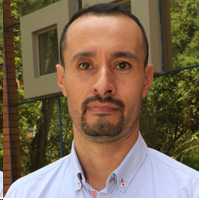
\includegraphics[keepaspectratio]{images/FAOM.png}}

\section*{Fredy Alejandro Ortiz
Meneses}\label{fredy-alejandro-ortiz-meneses}
\addcontentsline{toc}{section}{Fredy Alejandro Ortiz Meneses}

\markright{Fredy Alejandro Ortiz Meneses}

Microbiólogo con énfasis en Alimentos, Especialista en Pedagogía y
Didácticas Específicas, y Magíster en Fitopatología.

\end{tcolorbox}

\begin{tcolorbox}[enhanced jigsaw, toptitle=1mm, colbacktitle=quarto-callout-tip-color!10!white, breakable, opacityback=0, toprule=.15mm, coltitle=black, colframe=quarto-callout-tip-color-frame, bottomtitle=1mm, bottomrule=.15mm, titlerule=0mm, title=\textcolor{quarto-callout-tip-color}{\faLightbulb}\hspace{0.5em}{Tip}, colback=white, arc=.35mm, rightrule=.15mm, leftrule=.75mm, left=2mm, opacitybacktitle=0.6]

\pandocbounded{
\includegraphics[keepaspectratio]{images/MOPP.jpg}}

\section*{Miguel Oswaldo Pérez
Pulido}\label{miguel-oswaldo-puxe9rez-pulido}
\addcontentsline{toc}{section}{Miguel Oswaldo Pérez Pulido}

\markright{Miguel Oswaldo Pérez Pulido}

Director de Analítica Académica. Licenciado en Matemáticas y Magíster en
Estadística. Actualmente se desempeña como Director de Analítica
Académica, adscrito a la Vicerrectoría de Enseñanza. Está vinculado a la
Universidad de Santander (UDES) desde 2011, donde ha sido docente en
programas de pregrado y posgrado de la Facultad de Ciencias Exactas,
Naturales y Agropecuarias. Es investigador Junior reconocido por
Minciencias en la convocatoria 894 de 2021 y miembro del grupo de
investigación CIBAS

\end{tcolorbox}

\begin{tcolorbox}[enhanced jigsaw, toptitle=1mm, colbacktitle=quarto-callout-tip-color!10!white, breakable, opacityback=0, toprule=.15mm, coltitle=black, colframe=quarto-callout-tip-color-frame, bottomtitle=1mm, bottomrule=.15mm, titlerule=0mm, title=\textcolor{quarto-callout-tip-color}{\faLightbulb}\hspace{0.5em}{Tip}, colback=white, arc=.35mm, rightrule=.15mm, leftrule=.75mm, left=2mm, opacitybacktitle=0.6]

\pandocbounded{
\includegraphics[keepaspectratio]{images/FJL.jpg}}

\section*{Francisco Javier León}\label{francisco-javier-leuxf3n}
\addcontentsline{toc}{section}{Francisco Javier León}

\markright{Francisco Javier León}

Bacteriólogo y laboratorista clínico, con formación avanzada como
Magíster en Estadística Aplicada, Magíster en Ciencias Básicas
Biomédicas y Especialista en Educación con Nuevas Tecnologías. Está
vinculado a la Universidad de Santander (UDES) desde 2007, donde ha sido
docente en la Facultad de Ciencias Exactas, Naturales y Agropecuarias.
Actualmente, se desempeña como Coordinador de Analítica Académica,
adscrito a la Vicerrectoría de Enseñanza. Es investigador Junior
reconocido por Minciencias en la convocatoria 894 de 2021 y miembro del
grupo de investigación CIBAS

\end{tcolorbox}

\bookmarksetup{startatroot}

\chapter*{Agradecimientos}\label{agradecimientos}
\addcontentsline{toc}{chapter}{Agradecimientos}

\markboth{Agradecimientos}{Agradecimientos}

Queremos agradecer a Dios y nuestro más sincero reconocimiento a todos
los estudiantes y profesores del programa de Microbiología que, a lo
largo del tiempo, han compartido con nosotros sus inquietudes y retos al
intentar conectar el análisis estadístico con la microbiología
industrial.

Nuestro agradecimiento se extiende a los colegas académicos,
especialmente a los profesores Christian Andrey Chacín Zambrano y Daniel
Adyro Martinez; y a los estudiantes graduados que generosamente
compartieron sus experiencias y bases de datos, provenientes de
importantes experimentos académicos. Sus aportes han sido fundamentales
para dar vida a este manual y hacerlo relevante y aplicable a
situaciones reales dentro del contexto de la microbiología industrial.

Asimismo, manifestamos gratitud a Robert Gentleman y Ross Ihaka,
creadores del software R, así como a todos los colaboradores de la
comunidad de R y RStudio®. Gracias a su compromiso y dedicación, estas
herramientas se han mantenido accesibles para la comunidad científica.

A la Universidad de Santander (UDES) y a su Departamento de Desarrollo
Profesoral, por la apertura de la Convocatoria Interna de Producción de
Material Profesoral (2025). Esta valiosa iniciativa nos ha brindado un
espacio de apoyo institucional que reconoce y valora la creación de
material educativo de calidad. Gracias a ello, nos sentimos motivados a
seguir desarrollando herramientas que fortalezcan una enseñanza efectiva
en los campos de la Microbiología Industrial y la Estadística Aplicada.

\bookmarksetup{startatroot}

\chapter{Introducción}\label{introducciuxf3n}

El software R es un entorno y lenguaje de programación ampliamente
utilizado para el análisis estadístico y la visualización de datos, su
flexibilidad y capacidad para manejar grandes conjuntos de datos lo han
convertido en una herramienta esencial en la investigación científica,~
especialmente en campos como la microbiología industrial, donde el
análisis de datos es crucial para la optimización de procesos y la toma
de decisiones informadas; además de lo anterior, R ofrece una amplia
gama de paquetes y funciones que permiten realizar análisis complejos de
manera eficiente, facilitando la interpretación de resultados
experimentales (R Core Team 2021).

Por otra parte,
\href{https://posit.co/download/rstudio-desktop/}{RStudio®} es una
Interfaz de Desarrollo Integrada (IDE) para R que mejora
significativamente la experiencia del usuario, proporcionando un entorno
amigable y accesible para la programación y el análisis de datos, con
RStudio® los usuarios pueden escribir y ejecutar código, visualizar
gráficos y gestionar proyectos de manera más eficiente, lo que facilita
el aprendizaje y la aplicación de R en contextos académicos e
industriales (R Core Team 2021); cabe destacar que la combinación de
\href{https://www.r-project.org/}{R} y
\href{https://posit.co/download/rstudio-desktop/}{RStudio®} permite a
los estudiantes y profesionales de la microbiología industrial realizar
análisis estadísticos avanzados con mayor facilidad y precisión.

Una de las principales ventajas de
\href{https://posit.co/download/rstudio-desktop/}{RStudio®} es su
capacidad para integrar múltiples herramientas y recursos en una sola
plataforma, esto incluye: (i) un editor de código avanzado, (ii) una
consola interactiva, y (iii) herramientas de visualización de datos;
además de que RStudio® permite la instalación y gestión de paquetes
adicionales, lo que amplía sus funcionalidades y permite a los usuarios
personalizar su entorno de trabajo según sus necesidades (RStudio Team,
2023) (R Core Team 2021); esta flexibilidad es especialmente útil en la
microbiología industrial, donde los requisitos de análisis pueden variar
ampliamente según el tipo de experimento y los objetivos de
investigación.

Es importante destacar que el uso de R y RStudio® en la microbiología
industrial también promueve la reproducibilidad y transparencia en la
investigación; al utilizar un lenguaje de programación abierto y
ampliamente adoptado, los investigadores pueden compartir sus scripts y
métodos con la comunidad científica, lo que permite la verificación y
replicación de resultados, lo cual es fundamental para el avance del
conocimiento científico y la mejora continua de los procesos
industriales; además, la comunidad de usuarios de
\href{https://www.r-project.org/}{R} y
\href{https://posit.co/download/rstudio-desktop/}{RStudio} es muy
activa, lo que significa que los estudiantes y profesionales pueden
acceder a una gran cantidad de recursos y soporte en línea (Peng 2011).

En este libro, nos enfocaremos en cómo utilizar
\href{https://www.r-project.org/}{R} y
\href{https://posit.co/download/rstudio-desktop/}{RStudio®} para abordar
problemas específicos de la microbiología industrial; comenzaremos con
una introducción a la instalación y configuración de ambos programas,
seguida de una exploración de los paquetes esenciales para el análisis
de datos en microbiología; a lo largo del libro, proporcionaremos
ejemplos prácticos y estudios de caso que ilustran cómo aplicar estas
herramientas en situaciones reales; esto permitirá a los lectores
desarrollar una comprensión profunda y práctica de cómo utilizar
\href{https://www.r-project.org/}{R} y
\href{https://posit.co/download/rstudio-desktop/}{RStudio®} en su
trabajo diario (Grolemund and Wickham 2017).

\textbf{Referencias}

Peng, R. D. (2011). Reproducible research in computational science.
Science, 334(6060), 1226-1227.
\url{https://doi.org/10.1126/science.1213847}

R Core Team. (2023). R: A language and environment for statistical
computing. R Foundation for Statistical Computing.
\url{https://www.r-project.org}

RStudio Team. (2023). RStudio: Integrated Development for R. RStudio,
PBC. \url{https://posit.co/download/rstudio-desktop/}

Wickham, H., \& Grolemund, G. (2017). R for Data Science: Import, Tidy,
Transform, Visualize, and Model Data. O'Reilly Media.
\href{https://r4ds.had.co.nz/}{https://r4ds.had.co.nz}.

\bookmarksetup{startatroot}

\chapter{Summary}\label{summary}

Posible Reorganización:

• Prefacio • Autores • Agradecimientos • Introducción (Mantener como
introducción general al tema del libro)

\textbf{Parte I: Preparación del Entorno y Herramientas} • Instalación y
configuración de R y RStudio® (Lógica para comenzar con la configuración
del software) • Inventario de librerías básicas de R aplicadas para
análisis de datos (Después de la instalación, presentar las herramientas
fundamentales) • Paquetes Esenciales para el Análisis de Datos (Extender
las librerías básicas con paquetes clave)

\textbf{Parte II: Aplicaciones de R en Microbiología Industrial y
Análisis de Datos} • Uso de R en Microbiología Industrial (Presentar la
aplicación específica de R en tu campo) • Análisis Bibliométrico con
RStudio® (Un ejemplo concreto de análisis de datos con R) • Fundamentos
del Diseño Experimental (Introducir los principios del diseño
experimental) • Tipos de diseños experimentales (Expandir sobre los
diferentes tipos de diseños) • Diseño de experimentos en RStudio®
(Aplicar los conceptos de diseño experimental en R)

\textbf{Parte III: Gestión y Presentación de la Información} • Gestión
de la información con informes dinámicos (Conectar el análisis de datos
con la creación de informes)

References

\begin{tcolorbox}[enhanced jigsaw, toptitle=1mm, colbacktitle=quarto-callout-note-color!10!white, breakable, opacityback=0, toprule=.15mm, coltitle=black, colframe=quarto-callout-note-color-frame, bottomtitle=1mm, bottomrule=.15mm, titlerule=0mm, title=\textcolor{quarto-callout-note-color}{\faInfo}\hspace{0.5em}{Note}, colback=white, arc=.35mm, rightrule=.15mm, leftrule=.75mm, left=2mm, opacitybacktitle=0.6]

Este manual representa nuestra contribución a su formación integral como
científicos. Esperamos que no solo enriquezca su experiencia académica,
sino que también les proporcione las habilidades prácticas necesarias
para enfrentar los desafíos actuales y futuros del campo.

\end{tcolorbox}

\begin{tcolorbox}[enhanced jigsaw, toptitle=1mm, colbacktitle=quarto-callout-tip-color!10!white, breakable, opacityback=0, toprule=.15mm, coltitle=black, colframe=quarto-callout-tip-color-frame, bottomtitle=1mm, bottomrule=.15mm, titlerule=0mm, title=\textcolor{quarto-callout-tip-color}{\faLightbulb}\hspace{0.5em}{Using the data without downloading it}, colback=white, arc=.35mm, rightrule=.15mm, leftrule=.75mm, left=2mm, opacitybacktitle=0.6]

This same dataset is also available in the package palmerpenguins.

\end{tcolorbox}

\begin{tcolorbox}[enhanced jigsaw, toptitle=1mm, colbacktitle=quarto-callout-tip-color!10!white, breakable, opacityback=0, toprule=.15mm, coltitle=black, colframe=quarto-callout-tip-color-frame, bottomtitle=1mm, bottomrule=.15mm, titlerule=0mm, title=\textcolor{quarto-callout-tip-color}{\faLightbulb}\hspace{0.5em}{Título del Tip}, colback=white, arc=.35mm, rightrule=.15mm, leftrule=.75mm, left=2mm, opacitybacktitle=0.6]

Texto del contenido o recomendación.

\end{tcolorbox}

Tipos comunes de callouts:

\begin{verbatim}
callout-note → Para notas informativas.

callout-tip → Para consejos o buenas prácticas.

callout-warning → Para advertencias.

callout-important → Para contenido crítico o destacado.

callout-caution → Para precauciones.
\end{verbatim}

\begin{tcolorbox}[enhanced jigsaw, toptitle=1mm, colbacktitle=quarto-callout-warning-color!10!white, breakable, opacityback=0, toprule=.15mm, coltitle=black, colframe=quarto-callout-warning-color-frame, bottomtitle=1mm, bottomrule=.15mm, titlerule=0mm, title=\textcolor{quarto-callout-warning-color}{\faExclamationTriangle}\hspace{0.5em}{Cuidado}, colback=white, arc=.35mm, rightrule=.15mm, leftrule=.75mm, left=2mm, opacitybacktitle=0.6]

Este análisis puede producir resultados erróneos si no se limpian los
datos previamente.

\end{tcolorbox}

To learn more about Quarto books visit
\url{https://quarto.org/docs/books}.

\texttt{\{r\}\ 1\ +\ 1\}}

\bookmarksetup{startatroot}

\chapter{Parte I: Preparación del Entorno y
Herramientas}\label{parte-i-preparaciuxf3n-del-entorno-y-herramientas}

\section{3. Introducción al software R y
RStudio}\label{introducciuxf3n-al-software-r-y-rstudio}

\subsection{3.1 Instalación y
configuración}\label{instalaciuxf3n-y-configuraciuxf3n}

La instalación de R y RStudio® es un proceso sencillo que puede
completarse en unos pocos pasos; primero, se debe descargar e instalar R
desde el sitio web oficial del Proyecto R
(\url{https://www.r-project.org}); una vez instalado R, se puede
proceder a descargar e instalar RStudio® desde su sitio web
(\url{https://posit.co/download/rstudio-desktop/}) (Figura 1); ambos
programas están disponibles para múltiples sistemas operativos,
incluyendo Windows, macOS y Linux (Figura 2), del mismo modo se deben
descarga de diferentes directorios llamadas CRAN (Comprehensive R
Archive Network o Red integral de archivo R) (Figura 3); y finalmente
descargar la última compilación de R para Windows (Figura 4)
\href{R\%20Core\%20Team,\%202023}{@Rcore2021}.

Una vez instalados R y RStudio®, es importante familiarizarse con la
interfaz de RStudio® (Figura 5); esta interfaz está dividida en varias
secciones, incluyendo: (i) el editor de código o Script, el cual permite
escribir y editar las instrucciones o Scripts; (ii) la consola: se
utiliza para ejecutar comandos interactivos; ~(iii) el entorno de
trabajo: muestra los objetos y datos cargados en la sesión actual y las
(iv) pestañas de archivos y gráficos: permiten gestionar archivos y
visualizar gráficos generados por R (R Core Team 2021).

Además de la interfaz básica, RStudio® permite la instalación y gestión
de paquetes adicionales que amplían sus funcionalidades; para instalar
un paquete, se puede utilizar la función install.packages
(``nombre\_del\_paquete'') en la consola de RStudio®; una vez instalado,
el paquete se puede cargar en la sesión actual utilizando la función
library (nombre\_del\_paquete).

\begin{tcolorbox}[enhanced jigsaw, toptitle=1mm, colbacktitle=quarto-callout-important-color!10!white, breakable, opacityback=0, toprule=.15mm, coltitle=black, colframe=quarto-callout-important-color-frame, bottomtitle=1mm, bottomrule=.15mm, titlerule=0mm, title=\textcolor{quarto-callout-important-color}{\faExclamation}\hspace{0.5em}{Important}, colback=white, arc=.35mm, rightrule=.15mm, leftrule=.75mm, left=2mm, opacitybacktitle=0.6]

Mantener R y RStudio® actualizados es clave para aprovechar las últimas
mejoras, nuevas funcionalidades y correcciones de errores. Ambos
programas notifican automáticamente cuando hay versiones más recientes
disponibles, por lo que se recomienda estar atento a estos avisos y
actualizar oportunamente.

\end{tcolorbox}

Para actualizar R, se debe descargar e instalar la nueva versión desde
el sitio web del Proyecto R; para actualizar RStudio®, se puede utilizar
la opción de actualización en el menú de ayuda de RStudio®; mantener el
software actualizado garantiza un rendimiento óptimo y acceso a las
últimas funcionalidades (R Core Team 2021) (R Core Team, 2023; RStudio
Team, 2023).

~\textbf{Referencias}

R Core Team. (2023). R: A language and environment for statistical
computing. R Foundation for Statistical Computing.
\url{https://www.r-project.org}

RStudio Team. (2023). RStudio: Integrated Development for R. RStudio,
PBC. \url{https://posit.co/download/rstudio-desktop/}

Wickham, H. (2016). ggplot2: Elegant graphics for data analysis.
Springer. \url{https://doi.org/10.1007/978-3-319-24277-4}

Wickham, H., \& Grolemund, G. (2017). R for Data Science: Import, Tidy,
Transform, Visualize, and Model Data. O'Reilly Media.
\href{https://r4ds.had.co.nz/}{https://r4ds.had.co.nz}

\subsection{3.2 Paquetes Esenciales para el análisis de
datos}\label{paquetes-esenciales-para-el-anuxe1lisis-de-datos}

\subsubsection{Inventario de librerías básicas de R aplicadas para
análisis de datos (Unificar con el
siguiente)}\label{inventario-de-libreruxedas-buxe1sicas-de-r-aplicadas-para-anuxe1lisis-de-datos-unificar-con-el-siguiente}

En el ámbito de la microbiología industrial, el dominio de las librerías
básicas de R resulta fundamental para transformar datos experimentales
en información valiosa que guíe procesos industriales y decisiones
científicas, tal es el caso de la
\href{https://cran.r-project.org/web/packages/readxl/index.html}{librería
\emph{readxl}}, la cual fue desarrollada por (Wickham and Bryan 2015) y
es indispensable para la importación de datos desde hojas de cálculo
como Excel® (donde habitualmente los microbiólogos registran sus
resultados), facilitando la transferencia de información para
posteriormete ser tomada por el Script.

Por otro lado, la librería \emph{car} (Companion to Applied Regression),
creada por Fox y Weisberg (2019), ofrece herramientas esenciales para la
verificación de supuestos estadísticos, especialmente a través de
gráficos QQ-plot que permiten evaluar la normalidad de los datos
registrados, un requisito fundamental antes de aplicar a: pruebas
estadísticas paramétricas, aplicada en experimentos de optimización,
evaluación de medios de medios de cultivo, comparación de cepas
microbianas, entre otros.

Por su parte el paquete \emph{tidyverse} desarrollado por Wickham et
al.~(2019) representa una revolución en el análisis de datos
microbiológicos al integrar diversas librerías que comparten una lógica
común de programación y estructura de datos; este conjunto de
herramientas incluye librerías como: (i) \emph{dplyr} para manipulación
de datos, (ii) \emph{ggplot2} para visualización, (iii) \emph{tidyr}
para ordenamiento y (iv) \emph{readr} para importación, facilita
enormemente el flujo de trabajo en análisis de datos complejos típicos
de la microbiología industrial; por ejemplo, en estudios de cinética
enzimática o de crecimiento microbiano, donde es necesario filtrar,
transformar y visualizar datos procedentes de múltiples réplicas y
condiciones experimentales.

Otra importante librería utilizada dentro del ecosistema de RStudio® es
\emph{apaTables} creada por Stanley (2021) la cual permite la generación
automática de tablas con formato APA directamente desde los análisis
estadísticos realizados en R, lo que facilita enormemente la
documentación rigurosa de resultados experimentales para publicaciones
científicas en el campo de la microbiología, ahorrando tiempo y
reduciendo errores en la presentación de datos complejos.

La representación visual efectiva de datos microbiológicos resulta
crucial para interpretar resultados y comunicar hallazgos, siendo la
librería \emph{gridExtra}, desarrollada por Auguie (2017) una
herramienta potente que permite la organización de múltiples gráficos en
una sola visualización, facilitando comparaciones entre diferentes
condiciones experimentales, microorganismos o variables respuesta;
asimismo la librería \emph{lsr} (Learning Statistics with R) creada por
Navarro (2015) ~proporciona funciones accesibles para realizar análisis
estadísticos fundamentales en investigaciones microbiológicas, como:
pruebas t, ANOVA y cálculos de tamaño del efecto, facilitando la
interpretación de la significancia práctica de los resultados más allá
de la mera significancia estadística.

La evolución acelerada del conocimiento en Microbiología Industrial
requiere herramientas que permitan mantenerse actualizado con la
literatura científica, siendo la librería \emph{bibliometrix},
desarrollada por Aria y Cuccurullo (2017) el cual facilita el análisis
bibliométrico de publicaciones científicas, dicha librería permite
identificar: tendencias emergentes, autores influyentes y redes de
colaboración entre otras; proporcionando mapas de conocimiento que
orientan nuevas investigaciones e identifican vacíos en la literatura,
adicionalmente, permite a los investigadores contextualizar sus
hallazgos dentro del panorama científico global, potenciando la
relevancia e impacto de sus contribuciones científicas.

Al expandir nuestro arsenal analítico, encontramos librerías
especializadas que abordan necesidades específicas de la investigación
microbiológica industrial, como \emph{vegan} desarrollado por Oksanen et
al., (2020) la cual proporciona herramientas para análisis multivariado
y de diversidad ecológica; como son:~ los análisis de ordenación como
PCA (Análisis de Componentes Principales), NMDS (Escalamiento
Multidimensional No Métrico) y análisis de correspondencia canónica,
permitiendo visualizar relaciones complejas entre especies microbianas y
variables ambientales, parámetros que permiten estudiar comunidades
microbianas en procesos industriales como tratamiento de aguas
residuales, producción de biogás o fermentaciones alimentarias;

Por otra parte, la librería \emph{nlme} (Pinheiro et al., 2025) ofrece
capacidades para modelar datos longitudinales y con estructura
jerárquica, como los generados en estudios de cinética microbiana con
mediciones repetidas en el tiempo, permitiendo ajustar modelos mixtos
lineales y no lineales que capturan adecuadamente la variabilidad y
correlación temporal presentes en estos experimentos.

\textbf{Referencias}

Aria, M., \& Cuccurullo, C. (2017). bibliometrix: An R-tool for
comprehensive science mapping analysis. Journal of Informetrics, 11(4),
959-975. \url{https://doi.org/10.1016/j.joi.2017.08.007}

Auguie, B. (2017). gridExtra: Miscellaneous Functions for ``Grid''
Graphics. R package version 2.3.
\url{https://CRAN.R-project.org/package=gridExtra}

Fox, J., \& Weisberg, S. (2019). An R Companion to Applied Regression
(3rd ed.). Sage Publications.
\url{https://uk.sagepub.com/en-gb/eur/an-r-companion-to-applied-regression/book246125}

Gómez-Rubio, V. (2017). ggplot2 - Elegant Graphics for Data Analysis
(2nd Edition). Journal of Statistical Software, 77(Book Review 2), 1-3.
\url{https://doi.org/10.18637/jss.v077.b02}

Hardwicke, T. E., Mathur, M. B., MacDonald, K., Nilsonne, G., Banks, G.
C., Kidwell, M. C., Hofelich Mohr, A., Clayton, E., Yoon, E. J., Henry
Tessler, M., Lenne, R. L., Altman, S., Long, B., \& Frank, M. C. (2018).
Data availability, reusability, and analytic reproducibility: Evaluating
the impact of a mandatory open data policy at the journal Cognition.
Royal Society Open Science, 5(8), 180448.
\url{https://doi.org/10.1098/rsos.180448}

Navarro, D. J. (2015). Learning Statistics with R: A tutorial for
psychology students and other beginners. (Version 0.5). University of
Adelaide. \url{https://learningstatisticswithr.com/}

Oksanen, J., Blanchet, F. G., Friendly, M., Kindt, R., Legendre, P.,
McGlinn, D., Minchin, P. R., O'Hara, R. B., Simpson, G. L., Solymos, P.,
Stevens, M. H. H., Szoecs, E., \& Wagner, H. (2020). vegan: Community
ecology package. R package version 2.5-7.
\url{https://CRAN.R-project.org/package=vegan}

Pinheiro, J., Bates, D., DebRoy, S., Sarkar, D., \& R Core Team. (2025).
nlme: Linear and nonlinear mixed effects models. R package version
3.1-157. \url{https://CRAN.R-project.org/package=nlme}

Stanley, D. (2021). apaTables: Create American Psychological Association
(APA) Style Tables. R package version 2.0.8.
\url{https://CRAN.R-project.org/package=apaTables}

Wickham, H., \& Bryan, J. (2023). readxl: Read Excel Files. R package
version 1.4.2. \url{https://CRAN.R-project.org/package=readxl}

Wickham, H., Averick, M., Bryan, J., Chang, W., McGowan, L. D.,
François, R., Grolemund, G., Hayes, A., Henry, L., Hester, J., Kuhn, M.,
Pedersen, T. L., Miller, E., Bache, S. M., Müller, K., Ooms, J.,
Robinson, D., Seidel, D. P., Spinu, V., ... Yutani, H. (2019). Welcome
to the tidyverse. Journal of Open Source Software, 4(43), 1686.
\url{https://doi.org/10.21105/joss.01686}

\subsubsection{Paquetes Esenciales para el Análisis de Datos (Unificar
con el
anterior)}\label{paquetes-esenciales-para-el-anuxe1lisis-de-datos-unificar-con-el-anterior}

En el contexto de la microbiología industrial, el uso de paquetes
específicos en RStudio® es fundamental para realizar análisis de datos
de manera eficiente y precisa; uno de los paquetes más importantes es
tidyverse, que es una colección de paquetes diseñados para la
manipulación y limpieza de datos; tidyverse incluye herramientas como
\emph{dplyr} para la manipulación de datos\emph{, tidyr} para la
limpieza de datos y \emph{readr} para la importación de datos, lo que
facilita el manejo de grandes conjuntos de datos experimentales
(Wickham, 2017).

Otro paquete esencial es \emph{ggplot2}, que se utiliza para la
visualización de datos; \emph{ggplot2} permite crear gráficos complejos
y personalizados de manera sencilla, lo que es crucial para interpretar
y comunicar los resultados de los experimentos microbiológicos; la
capacidad de ggplot2 para generar gráficos de alta calidad ayuda a los
investigadores a identificar patrones y tendencias en los datos,
mejorando así la toma de decisiones en procesos industriales (Wickham,
2016).

El paquete dplyr es especialmente útil para el procesamiento de datos;
\emph{dplyr} proporciona una gramática coherente para la manipulación de
datos, permitiendo realizar operaciones como la selección, filtrado,
agrupamiento y resumen de datos de manera eficiente; estas funciones son
esenciales para preparar los datos antes de realizar análisis
estadísticos más avanzados, asegurando que los datos estén en el formato
adecuado para su análisis (Wickham, 2017) (Wickham 2016).

Para el diseño de experimentos, el paquete \emph{agricolae} es una
herramienta valiosa; aunque originalmente desarrollado para ciencias
agrícolas, \emph{agricolae} ofrece funciones que son igualmente
aplicables en la microbiología industrial; este paquete permite crear
diseños experimentales como bloques completos aleatorizados, diseños
factoriales y análisis de varianza (ANOVA), facilitando la planificación
y análisis de experimentos complejos (Mendiburu, 2020).

Finalmente, el paquete \emph{shiny} permite la creación de aplicaciones
web interactivas; \emph{shiny} es especialmente útil para desarrollar
herramientas que permitan a los investigadores interactuar con sus datos
de manera dinámica; estas aplicaciones pueden ser utilizadas para
visualizar resultados en tiempo real, realizar análisis exploratorios y
compartir hallazgos con colegas y la comunidad científica, mejorando la
colaboración y la transparencia en la investigación (Chang et al.,
2021).

\textbf{Referencias}

Chang, W., Cheng, J., Allaire, J., Xie, Y., \& McPherson, J. (2021).
shiny: Web Application Framework for R. R package version 1.6.0.
\url{https://CRAN.R-project.org/package=shiny}

Mendiburu, F. (2020). agricolae: Statistical Procedures for Agricultural
Research. R package version 1.3-3.
\url{https://CRAN.R-project.org/package=agricolae}

Wickham, H. (2016). ggplot2: Elegant graphics for data analysis.
Springer. \url{https://doi.org/10.1007/978-3-319-24277-4}

Wickham, H. (2017). tidyverse: Easily Install and Load the `Tidyverse'.
R package version 1.2.1.
\url{https://CRAN.R-project.org/package=tidyverse}

Wickham, H., \& Grolemund, G. (2017). R for Data Science: Import, Tidy,
Transform, Visualize, and Model Data. O'Reilly Media.
\url{https://r4ds.had.co.nz}

\subsubsection{Uso de R en Microbiología
Industrial}\label{uso-de-r-en-microbiologuxeda-industrial}

El uso de R como herramienta de análisis estadístico en la microbiología
industrial ha experimentado un crecimiento exponencial en la última
década, según Mohammadi et al.~(2019) R proporciona una plataforma
versátil que permite analizar datos complejos derivados de experimentos
microbiológicos, facilitando la identificación de patrones de
crecimiento microbiano, optimización de condiciones de cultivo y
evaluación de la producción de metabolitos secundarios, lo que resulta
crucial para el desarrollo y mejora de procesos biotecnológicos en
entornos industriales.

McMurdie y Holmes (2013) desarrollaron el paquete \emph{phyloseq}, el
cual ha transformado el análisis de datos de secuenciación en estudios
de comunidades microbianas, permitiendo la integración de información
taxonómica, filogenética y de abundancia en un solo entorno analítico;
este avance ha sido fundamental para comprender la dinámica de
poblaciones microbianas en procesos industriales como: el tratamiento de
aguas residuales, la producción de biocombustibles y la fermentación
alimentaria.

Por otra parte, el paquete microbiome, descrito por Lahti y Shetty
(2017) (Reeder et al. 2021), proporciona herramientas especializadas
para el análisis de datos metagenómicos, facilitando la caracterización
de comunidades microbianas y sus funciones metabólicas en entornos
industriales, lo que resulta esencial para la optimización de
bioprocesos y el control de calidad en la industria alimentaria.

El diseño experimental en microbiología industrial se ha beneficiado
significativamente de la aplicabilidad de R, permitiendo planificar y
analizar experimentos de manera más rigurosa y eficiente, el paquete
\emph{agricolae}, desarrollado por de Mendiburu (2021) (Zhou et al.
2012) es utilizado para la implementación de diseños experimentales
complejos como: bloques aleatorizados y diseños factoriales entre otros,
al tiempo que frecuentemente son utilizados en estudios de optimización
de medios de cultivo, condiciones de fermentación y producción de
enzimas microbianas.

Complementariamente, Ritz y Streibig (2005) presentaron el paquete
\emph{drc} (Dose-Response Curves), que ha facilitado el análisis de
Curvas dosis-respuesta en estudios de inhibición microbiana, pruebas de
susceptibilidad a antimicrobianos y evaluación de compuestos bioactivos
producidos por microorganismos, proporcionando herramientas estadísticas
robustas para cuantificar y modelar respuestas biológicas a diferentes
tratamientos, lo cual es fundamental en el desarrollo de nuevos
productos biotecnológicos.

Gracias al paquete \emph{ggplot2} desarrollado por Wickham (2016), el
cual ha permitido la creación de gráficos elegantes y altamente
informativos que facilitan la interpretación de resultados
experimentales; en particular, la representación gráfica de cinéticas de
crecimiento microbiano, producción de metabolitos y análisis
multivariantes se ha vuelto más accesible e intuitiva para
investigadores en el campo; de manera similar el paquete \emph{ggtree},
creado por Yu et al.~(2017), ha revolucionado la visualización de datos
filogenéticos en estudios de diversidad microbiana industrial,
permitiendo representar relaciones evolutivas entre microorganismos de
interés biotecnológico y correlacionarlas con características
fenotípicas relevantes para procesos industriales, lo que facilita la
selección de cepas microbianas con potencial biotecnológico.

\begin{tcolorbox}[enhanced jigsaw, toptitle=1mm, colbacktitle=quarto-callout-caution-color!10!white, breakable, opacityback=0, toprule=.15mm, coltitle=black, colframe=quarto-callout-caution-color-frame, bottomtitle=1mm, bottomrule=.15mm, titlerule=0mm, title=\textcolor{quarto-callout-caution-color}{\faFire}\hspace{0.5em}{Expandir para aprender son el analis de datos ómicos}, colback=white, arc=.35mm, rightrule=.15mm, leftrule=.75mm, left=2mm, opacitybacktitle=0.6]

El análisis de datos ómicos en microbiología industrial se ha visto
significativamente potenciado gracias al aporte de Love et al.~(2014)
quienes introdujeron \emph{DESeq2}, un paquete que ha transformado el
análisis de datos de RNA-seq en estudios transcriptómicos de
microorganismos industriales, permitiendo identificar genes
diferencialmente expresados bajo diversas condiciones de cultivo o
modificaciones genéticas; lo que contribuye a la mejora de cepas
microbianas industriales y a optimizar rutas metabólicas de interés
comercial; paralelamente Rohart et al.~(2017) desarrollaron el paquete
mixOmics, el cual facilita la integración de múltiples conjuntos de
datos ómicos, como:

\begin{enumerate}
\def\labelenumi{(\roman{enumi})}
\tightlist
\item
  transcriptómica,
\item
  proteómica y
\item
  metabolómica,
\end{enumerate}

proporcionando una visión holística de los sistemas microbianos en
contextos industriales, lo que permite desentrañar complejas redes
regulatorias y metabólicas que subyacen a procesos biotecnológicos
importantes como de compuestos bioactivos..

\end{tcolorbox}

\begin{tcolorbox}[enhanced jigsaw, toptitle=1mm, colbacktitle=quarto-callout-caution-color!10!white, breakable, opacityback=0, toprule=.15mm, coltitle=black, colframe=quarto-callout-caution-color-frame, bottomtitle=1mm, bottomrule=.15mm, titlerule=0mm, title=\textcolor{quarto-callout-caution-color}{\faFire}\hspace{0.5em}{Expand to learn more about where the data was collected}, colback=white, arc=.35mm, rightrule=.15mm, leftrule=.75mm, left=2mm, opacitybacktitle=0.6]

Data were collected and made available by Dr.~Kristen Gorman and the
Palmer Station, Antarctica LTER, a member of the Long Term Ecological
Research Network.

\end{tcolorbox}

\textbf{Referencias}

Zhou et al. (2012)

González-Peña, D., Dudzik, D., García, A., Legido-Quigley, C., \&
Barbas, C. (2021). R in LC-MS-based metabolomics: A review of packages,
tutorials, and case studies. Metabolites, 11(10), 672.
\url{https://doi.org/10.3390/metabo11100672} \textbf{\emph{Esta
referencia esta mal}}

\textbf{\emph{Zhou, B., Xiao, J. F., Tuli, L., \& Ressom, H. W. (2012).
LC-MS-based metabolomics. Molecular BioSystems, 8(2), 470--481.
https://doi.org/10.1039/c1mb05350g}} ( es esta ???)

Lahti, L., \& Shetty, S. (2017). microbiome R package. Tools Microbiome
Anal. R. \url{http://microbiome.github.io/microbiome}
\textbf{\emph{Cambiarla mejor por la que sigue???}}

\textbf{\emph{Reeder, J., Huang, M., Kaminker, J. S., \& Paulson, J. N.
(2021). MicrobiomeExplorer: an R package for the analysis and
visualization of microbial communities. Bioinformatics (Oxford,
England), 37(9), 1317--1318.
https://doi.org/10.1093/bioinformatics/btaa838}} ( es esta ???)

Love, M. I., Huber, W., \& Anders, S. (2014). Moderated estimation of
fold change and dispersion for RNA-seq data with DESeq2. Genome Biology,
15(12), 550. \url{https://doi.org/10.1186/s13059-014-0550-8}

McMurdie, P. J., \& Holmes, S. (2013). phyloseq: An R package for
reproducible interactive analysis and graphics of microbiome census
data. PLOS ONE, 8(4), e61217.
\url{https://doi.org/10.1371/journal.pone.0061217}

Mendiburu, F. (2021). agricolae: Statistical procedures for agricultural
research. R package version 1.4-0.
\url{https://CRAN.R-project.org/package=agricolae}

Mohammadi, R., Ghomi, S. M. T. F., \& Nazari, F. (2019). The application
of R software for the assessment of microbial fermentation processes.
Journal of Microbiological Methods, 156, 54-58.
\url{https://doi.org/10.1016/j.mimet.2018.12.003}

Ritz, C., \& Streibig, J. C. (2005). Bioassay analysis using R. Journal
of Statistical Software, 12(5), 1-22.
\url{https://doi.org/10.18637/jss.v012.i05}

Rohart, F., Gautier, B., Singh, A., \& Lê Cao, K. A. (2017). mixOmics:
An R package for 'omics feature selection and multiple data integration.
PLOS Computational Biology, 13(11), e1005752.
\url{https://doi.org/10.1371/journal.pcbi.1005752}

Wickham, H. (2016). ggplot2: Elegant graphics for data analysis (2nd
ed.). Springer. \url{https://doi.org/10.1007/978-3-319-24277-4}

Yu, G., Smith, D. K., Zhu, H., Guan, Y., \& Lam, T. T. Y. (2017).
ggtree: An R package for visualization and annotation of phylogenetic
trees with their covariates and other associated data. Methods in
Ecology and Evolution, 8(1), 28-36.
\url{https://doi.org/10.1111/2041-210X.12628}

\section{4. Análisis Bibliométrico con RStudio® (Un ejemplo concreto de
análisis de datos con
R)}\label{anuxe1lisis-bibliomuxe9trico-con-rstudio-un-ejemplo-concreto-de-anuxe1lisis-de-datos-con-r}

\bookmarksetup{startatroot}

\chapter{Parte II: Aplicaciones de R en Microbiología Industrial y
Análisis de
Datos}\label{parte-ii-aplicaciones-de-r-en-microbiologuxeda-industrial-y-anuxe1lisis-de-datos}

\section{2. Fundamentos del Diseño Experimental (Introducir los
principios del diseño experimental
OK)}\label{fundamentos-del-diseuxf1o-experimental-introducir-los-principios-del-diseuxf1o-experimental-ok}

\subsection{2.1 Tipos de diseños experimentales (Expandir sobre los
diferentes tipos de diseños
OK)}\label{tipos-de-diseuxf1os-experimentales-expandir-sobre-los-diferentes-tipos-de-diseuxf1os-ok}

\subsection{2.2 Ejemplos prácticos de diseños experimentales en
Microbiología Industrial
OK}\label{ejemplos-pruxe1cticos-de-diseuxf1os-experimentales-en-microbiologuxeda-industrial-ok}

\subsubsection{2.2.1 Diseño completamente al azar
OK}\label{diseuxf1o-completamente-al-azar-ok}

\begin{tcolorbox}[enhanced jigsaw, toptitle=1mm, colbacktitle=quarto-callout-important-color!10!white, breakable, opacityback=0, toprule=.15mm, coltitle=black, colframe=quarto-callout-important-color-frame, bottomtitle=1mm, bottomrule=.15mm, titlerule=0mm, title=\textcolor{quarto-callout-important-color}{\faExclamation}\hspace{0.5em}{Problema}, colback=white, arc=.35mm, rightrule=.15mm, leftrule=.75mm, left=2mm, opacitybacktitle=0.6]

Escibrir los datos del problema y la bibliografci de donde se saco la
información.

\end{tcolorbox}

\subsection{Estructura de la base de
datos}\label{estructura-de-la-base-de-datos}

La base de datos utilizada en este análisis corresponde a los resultados
de un experimento agrícola que evalúa el comportamiento de cuatro
cultivos diferentes bajo condiciones similares de manejo. La tabla
contiene tres columnas principales:

\begin{longtable}[]{@{}
  >{\raggedright\arraybackslash}p{(\linewidth - 2\tabcolsep) * \real{0.3194}}
  >{\raggedright\arraybackslash}p{(\linewidth - 2\tabcolsep) * \real{0.6806}}@{}}
\toprule\noalign{}
\begin{minipage}[b]{\linewidth}\raggedright
Variable
\end{minipage} & \begin{minipage}[b]{\linewidth}\raggedright
Descripción
\end{minipage} \\
\midrule\noalign{}
\endhead
\bottomrule\noalign{}
\endlastfoot
\texttt{Tratamiento} & Tipo de cultivo evaluado. Incluye cuatro niveles:
Arroz, Avena, Cebada y Maíz. \\
\texttt{Repetición} & Número de repetición del tratamiento (del 1 al 4).
Permite el análisis estadístico con replicación. \\
\texttt{Resultado} & Valor numérico correspondiente a la variable
respuesta medida (por ejemplo, rendimiento en kg/ha). \\
\end{longtable}

\textbf{Pasos para trabajar con R o RStudio:}

Especificar el directorio que me interesa donde se encuentra la base de
datos.

\begin{tcolorbox}[enhanced jigsaw, toptitle=1mm, colbacktitle=quarto-callout-tip-color!10!white, breakable, opacityback=0, toprule=.15mm, coltitle=black, colframe=quarto-callout-tip-color-frame, bottomtitle=1mm, bottomrule=.15mm, titlerule=0mm, title=\textcolor{quarto-callout-tip-color}{\faLightbulb}\hspace{0.5em}{Antes e inciar}, colback=white, arc=.35mm, rightrule=.15mm, leftrule=.75mm, left=2mm, opacitybacktitle=0.6]

R lee / (slash o division) y no el de Windows \textbackslash{}

En \textbf{R}, \texttt{setwd()} es una función que significa
\textbf{``set working directory''} o ``establecer el directorio de
trabajo''. Se utiliza para \textbf{definir la carpeta predeterminada} en
la que R buscará archivos para leer y donde guardará archivos por
defecto.\\

Por ejemplo: setwd (``D:/OneDrive - Universidad de Santander/Material
Docente 2025/CodigoR''\,``)

\end{tcolorbox}

\textbf{Lectura de datos}

\begin{Shaded}
\begin{Highlighting}[]
\FunctionTok{library}\NormalTok{(readxl)}
\end{Highlighting}
\end{Shaded}

\begin{verbatim}
Warning: package 'readxl' was built under R version 4.3.3
\end{verbatim}

\begin{Shaded}
\begin{Highlighting}[]
\NormalTok{DCA }\OtherTok{\textless{}{-}} \FunctionTok{read\_excel}\NormalTok{(}\StringTok{"C:/Users/coordinador.analitic/OneDrive {-} Universidad de Santander/Material\_Profesoral\_2025/CodigoR/DCA2.xlsx"}\NormalTok{)}

\FunctionTok{View}\NormalTok{(DCA)}
\FunctionTok{attach}\NormalTok{(DCA)}
\FunctionTok{names}\NormalTok{(DCA)}
\end{Highlighting}
\end{Shaded}

\begin{verbatim}
[1] "Tratamiento" "Repeticion"  "Resultado"  
\end{verbatim}

\begin{Shaded}
\begin{Highlighting}[]
\FunctionTok{str}\NormalTok{(DCA)}
\end{Highlighting}
\end{Shaded}

\begin{verbatim}
tibble [16 x 3] (S3: tbl_df/tbl/data.frame)
 $ Tratamiento: chr [1:16] "Arroz" "Arroz" "Arroz" "Arroz" ...
 $ Repeticion : num [1:16] 1 2 3 4 1 2 3 4 1 2 ...
 $ Resultado  : num [1:16] 8.76 8.74 8.72 8.72 8.39 ...
\end{verbatim}

\begin{Shaded}
\begin{Highlighting}[]
\FunctionTok{summary}\NormalTok{(DCA}\SpecialCharTok{$}\NormalTok{Resultado)}
\end{Highlighting}
\end{Shaded}

\begin{verbatim}
   Min. 1st Qu.  Median    Mean 3rd Qu.    Max. 
  8.341   8.635   8.792   8.775   8.954   9.141 
\end{verbatim}

\textbf{Análisis de la Varianza - ANOVA}

Cuando se desea saber si varios grupos (Ej. tratamientos) presentan
diferencias reales en sus promedios, una de las herramientas
estadísticas más utilizadas es el Análisis de la Varianza, conocido como
ANOVA. Esta técnica permite examinar si los valores medios de tres o más
grupos son lo suficientemente distintos como para concluir que no se
trata de simples fluctuaciones aleatorias.

El enfoque de ANOVA se basa en comparar dos tipos de variación: por un
lado, l\textbf{a variabilidad que se observa entre los distintos
grupos}, y por otro, \textbf{la variabilidad que existe dentro de cada
grupo individual}.

Si al analizar los datos se encuentra que la variación entre los grupos
supera notablemente la que ocurre dentro de ellos, es razonable pensar
que las diferencias en los promedios reflejan algo más que el azar. En
cambio, si la variabilidad interna es más pronunciada, entonces es
posible que las diferencias observadas no sean significativas y
respondan a variaciones normales del comportamiento de los datos.

\textbf{Código de R para ANOVA}

\begin{Shaded}
\begin{Highlighting}[]
\NormalTok{Anova}\OtherTok{\textless{}{-}}\FunctionTok{aov}\NormalTok{(Resultado}\SpecialCharTok{\textasciitilde{}}\NormalTok{Tratamiento, }\AttributeTok{data=}\NormalTok{DCA)}
\FunctionTok{summary}\NormalTok{(Anova)}
\end{Highlighting}
\end{Shaded}

\begin{verbatim}
            Df Sum Sq Mean Sq F value   Pr(>F)    
Tratamiento  3 1.1794  0.3931   660.4 1.39e-13 ***
Residuals   12 0.0071  0.0006                     
---
Signif. codes:  0 '***' 0.001 '**' 0.01 '*' 0.05 '.' 0.1 ' ' 1
\end{verbatim}

\textbf{Interpretación:} La prueba ANOVA muestra diferencias
significativas entre los tratamientos (p \textless{} 0.001). El valor de
F (660.4) indica que la variación entre tratamientos es mucho mayor que
la variación dentro de los grupos, lo que sugiere que al menos uno de
los tratamientos afecta significativamente el resultado.

\textbf{Modelo Lineal}

\begin{Shaded}
\begin{Highlighting}[]
\NormalTok{modelo}\OtherTok{=}\FunctionTok{lm}\NormalTok{(Resultado}\SpecialCharTok{\textasciitilde{}}\NormalTok{(Tratamiento))}
\FunctionTok{summary}\NormalTok{(modelo)}
\end{Highlighting}
\end{Shaded}

\begin{verbatim}

Call:
lm(formula = Resultado ~ (Tratamiento))

Residuals:
      Min        1Q    Median        3Q       Max 
-0.038397 -0.016205  0.001983  0.012013  0.040116 

Coefficients:
                  Estimate Std. Error t value Pr(>|t|)    
(Intercept)        8.73389    0.01220 715.921  < 2e-16 ***
TratamientoAvena  -0.35848    0.01725 -20.778 8.93e-11 ***
TratamientoCebada  0.12669    0.01725   7.343 8.94e-06 ***
TratamientoMaiz    0.39630    0.01725  22.970 2.75e-11 ***
---
Signif. codes:  0 '***' 0.001 '**' 0.01 '*' 0.05 '.' 0.1 ' ' 1

Residual standard error: 0.0244 on 12 degrees of freedom
Multiple R-squared:  0.994, Adjusted R-squared:  0.9925 
F-statistic: 660.4 on 3 and 12 DF,  p-value: 1.393e-13
\end{verbatim}

\textbf{Interpretación:} El modelo lineal confirma que el tratamiento
influye significativamente en los resultados (p \textless{} 0.001). El
tratamiento ``Arroz'' actúa como referencia, con una media estimada de
8.73. Comparado con este:

\begin{verbatim}
Avena presenta una media significativamente menor (–0.36, p < 0.001).

Cebada muestra un aumento moderado (+0.13, p < 0.001).

Maíz tiene el mayor incremento (+0.40, p < 0.001).
\end{verbatim}

El modelo explica el 99.4\% de la variabilidad en los datos (R² =
0.994), y el error estándar residual es bajo (0.0244), lo que indica un
ajuste excelente.

\textbf{Gráfico Boxplot}

Se toma el Tratamiento para hacer un boxplot utilizando la variable
``Resultado'', pero primero se transformar en factor la variable
Tratamiento:

\begin{Shaded}
\begin{Highlighting}[]
\FunctionTok{library}\NormalTok{(ggplot2)}

\NormalTok{DCA}\SpecialCharTok{$}\NormalTok{Treatamiento}\OtherTok{\textless{}{-}}\FunctionTok{factor}\NormalTok{(DCA}\SpecialCharTok{$}\NormalTok{Tratamiento) }\CommentTok{\#transformamos una variable númerica en un factor categórico}
\FunctionTok{ggplot}\NormalTok{(DCA, }\FunctionTok{aes}\NormalTok{(}\AttributeTok{x =}\NormalTok{ Tratamiento, }\AttributeTok{y =}\NormalTok{ Resultado, }\AttributeTok{fill=}\NormalTok{Tratamiento)) }\SpecialCharTok{+} 
  \FunctionTok{geom\_boxplot}\NormalTok{()}
\end{Highlighting}
\end{Shaded}

\pandocbounded{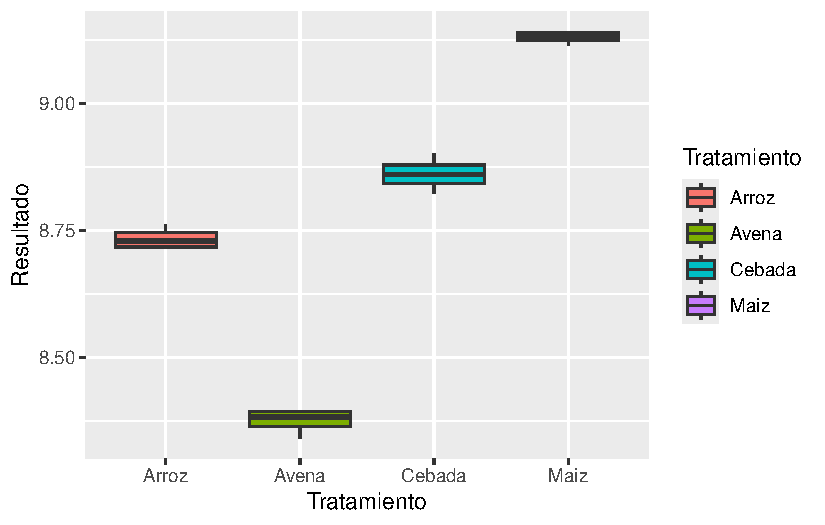
\includegraphics[keepaspectratio]{Chapter_02_files/figure-pdf/unnamed-chunk-4-1.pdf}}

\textbf{Interpretación:} Las diferencias en las medianas entre
tratamientos son claras y consistentes con los resultados del ANOVA y
del modelo lineal, lo que sugiere un efecto significativo del tipo de
cultivo sobre la variable resultado.

\textbf{Supuestos del diseño}

\textbf{Normalidad:} Para verificar la normalidad de los residuos
utilizaremos la prueba de Shapiro-Wilks cuyo script es el siguiente:

\begin{Shaded}
\begin{Highlighting}[]
\FunctionTok{shapiro.test}\NormalTok{(}\FunctionTok{residuals}\NormalTok{(Anova))}
\end{Highlighting}
\end{Shaded}

\begin{verbatim}

    Shapiro-Wilk normality test

data:  residuals(Anova)
W = 0.97944, p-value = 0.959
\end{verbatim}

\textbf{Interpretación:} El test de Shapiro-Wilk aplicado a los residuos
del modelo ANOVA devuelve un valor de p = 0.959, que es mucho mayor que
0.05. Esto indica que no hay evidencia estadística para rechazar la
hipótesis nula de normalidad. Por lo tanto, se concluye que los residuos
del modelo siguen una distribución normal, cumpliendo así uno de los
supuestos fundamentales del análisis de varianza.

\textbf{Gráficos para evaluar la normalidad}

Para construir el gráfico QQ (QQ plot) y evaluar la normalidad de los
datos, se utiliza la función correspondiente del paquete car. Si no está
instalado previamente, es necesario instalar también el paquete auxiliar
carData.

Instalación (si es necesario) install.packages (``car'')
install.packages (``carData'') install.packages (``dplyr'')
install.packages (``purrr'')

\textbf{Cargar los paquetes (librerias)}

\begin{Shaded}
\begin{Highlighting}[]
\FunctionTok{library}\NormalTok{(car) }\CommentTok{\#Grafico de QQ plot}
\FunctionTok{library}\NormalTok{(carData)}
\FunctionTok{library}\NormalTok{(dplyr)}
\FunctionTok{library}\NormalTok{(purrr)}

\FunctionTok{qqPlot}\NormalTok{(Anova)}
\end{Highlighting}
\end{Shaded}

\pandocbounded{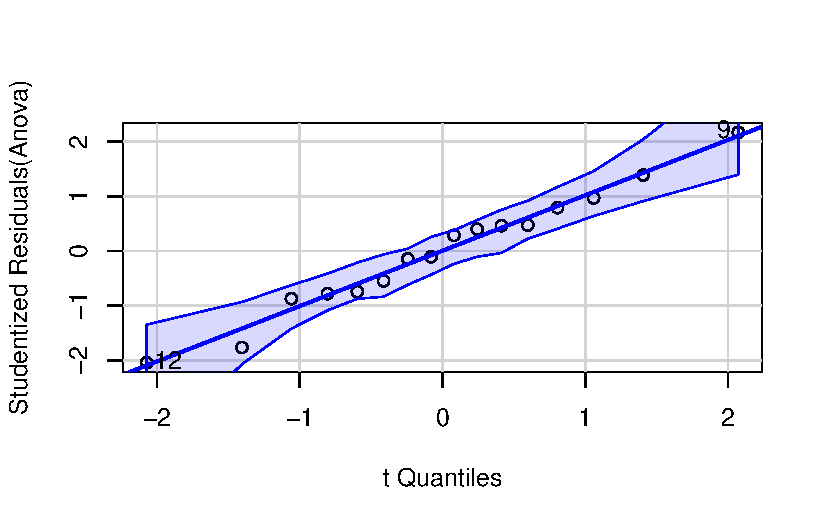
\includegraphics[keepaspectratio]{Chapter_02_files/figure-pdf/unnamed-chunk-6-1.pdf}}

\begin{verbatim}
[1]  9 12
\end{verbatim}

\textbf{Interpretación:} El gráfico QQ muestra que los residuos
estandarizados del modelo ANOVA se alinean adecuadamente con la línea
diagonal, lo que indica que su distribución es aproximadamente normal.
La mayoría de los puntos se ubican dentro de la banda de confianza, y no
se observan desviaciones sistemáticas. Esta gráfica complementa el
resultado del test de Shapiro-Wilk (p = 0.959), confirmando que se
cumple el supuesto de normalidad de los residuos en el modelo.

\textbf{Homocedasticidad:} Para evaluar el supuesto de homogeneidad de
varianzas entre los grupos (homocedasticidad), se aplicará la prueba de
Bartlett, la cual es apropiada cuando los datos provienen de poblaciones
aproximadamente normales. Esta prueba contrasta la hipótesis nula de
igualdad de varianzas frente a la alternativa de varianzas diferentes.
El procedimiento se implementa mediante el siguiente script:

\begin{Shaded}
\begin{Highlighting}[]
\FunctionTok{bartlett.test}\NormalTok{(Resultado}\SpecialCharTok{\textasciitilde{}}\NormalTok{Tratamiento, }\AttributeTok{data=}\NormalTok{DCA)}
\end{Highlighting}
\end{Shaded}

\begin{verbatim}

    Bartlett test of homogeneity of variances

data:  Resultado by Tratamiento
Bartlett's K-squared = 2.2722, df = 3, p-value = 0.5179
\end{verbatim}

\textbf{Interpretación:} Dado que el valor de p es mayor que 0.05 (p =
0.5179), no se rechaza la hipótesis nula. Por tanto, se asume que las
varianzas entre los tratamientos son homogéneas, cumpliéndose este
supuesto clave para el análisis de varianza y para la aplicación de
pruebas a posteriori como LSD.

\textbf{Pruebas aposteriori} Para identificar diferencias específicas
entre las medias de los tratamientos, una vez detectada significancia en
el análisis de varianza, se aplicará una prueba de comparaciones
múltiples a posteriori. En este caso, se empleará la técnica LSD (Least
Significant Difference), que permite realizar comparaciones pareadas
entre tratamientos asumiendo homogeneidad de varianzas.

La implementación de esta prueba requiere la carga del paquete
agricolae, utilizando el siguiente script. Instalación si es necesario:
install.packages(``agricolae''). Carga del paquete: library(agricolae).

\begin{Shaded}
\begin{Highlighting}[]
\FunctionTok{library}\NormalTok{(agricolae)}
\NormalTok{Grupos }\OtherTok{\textless{}{-}} \FunctionTok{LSD.test}\NormalTok{(}\AttributeTok{y =}\NormalTok{ Anova, }\AttributeTok{trt =} \StringTok{"Tratamiento"}\NormalTok{, }\AttributeTok{group =}\NormalTok{ T, }\AttributeTok{console =}\NormalTok{ T)}
\end{Highlighting}
\end{Shaded}

\begin{verbatim}

Study: Anova ~ "Tratamiento"

LSD t Test for Resultado 

Mean Square Error:  0.0005953124 

Tratamiento,  means and individual ( 95 %) CI

       Resultado        std r         se      LCL      UCL      Min      Max
Arroz   8.733890 0.02192214 4 0.01219951 8.707310 8.760471 8.715318 8.762183
Avena   8.375414 0.02519485 4 0.01219951 8.348834 8.401995 8.341039 8.395990
Cebada  8.860578 0.03330518 4 0.01219951 8.833998 8.887159 8.822181 8.900695
Maiz    9.130190 0.01251613 4 0.01219951 9.103609 9.156770 9.113429 9.140539
            Q25      Q50      Q75
Arroz  8.717232 8.729030 8.745688
Avena  8.364419 8.382314 8.393309
Cebada 8.842075 8.859719 8.878222
Maiz   9.124249 9.133395 9.139335

Alpha: 0.05 ; DF Error: 12
Critical Value of t: 2.178813 

least Significant Difference: 0.03759044 

Treatments with the same letter are not significantly different.

       Resultado groups
Maiz    9.130190      a
Cebada  8.860578      b
Arroz   8.733890      c
Avena   8.375414      d
\end{verbatim}

\textbf{Intrepretación:} La prueba LSD reveló que los cuatro
tratamientos presentan diferencias estadísticamente significativas entre
sus medias. El tratamiento Maíz obtuvo el mayor rendimiento promedio,
seguido por Cebada, Arroz y Avena, en ese orden descendente.

Otra opcion cuando cambiamos el argumento ``group'' a F(false), se
interpreta a mi parecer de forma mas sencilla la diferencia entre las
medias.A continuación, se presentan las pruebas de comparaciones
múltiples a posteriori aplicadas al modelo de ANOVA ajustado. Se
incluyen la prueba LSD, la prueba de Tukey y el test de Scheffé, las
cuales permiten identificar diferencias estadísticamente significativas
entre los tratamientos evaluados:

\begin{Shaded}
\begin{Highlighting}[]
\NormalTok{Grupos}\OtherTok{\textless{}{-}} \FunctionTok{LSD.test}\NormalTok{(}\AttributeTok{y =}\NormalTok{ Anova, }\AttributeTok{trt =} \StringTok{"Tratamiento"}\NormalTok{, }\AttributeTok{group =}\NormalTok{ F, }\AttributeTok{console =}\NormalTok{ T)}
\end{Highlighting}
\end{Shaded}

\begin{verbatim}

Study: Anova ~ "Tratamiento"

LSD t Test for Resultado 

Mean Square Error:  0.0005953124 

Tratamiento,  means and individual ( 95 %) CI

       Resultado        std r         se      LCL      UCL      Min      Max
Arroz   8.733890 0.02192214 4 0.01219951 8.707310 8.760471 8.715318 8.762183
Avena   8.375414 0.02519485 4 0.01219951 8.348834 8.401995 8.341039 8.395990
Cebada  8.860578 0.03330518 4 0.01219951 8.833998 8.887159 8.822181 8.900695
Maiz    9.130190 0.01251613 4 0.01219951 9.103609 9.156770 9.113429 9.140539
            Q25      Q50      Q75
Arroz  8.717232 8.729030 8.745688
Avena  8.364419 8.382314 8.393309
Cebada 8.842075 8.859719 8.878222
Maiz   9.124249 9.133395 9.139335

Alpha: 0.05 ; DF Error: 12
Critical Value of t: 2.178813 

Comparison between treatments means

               difference pvalue signif.        LCL         UCL
Arroz - Avena   0.3584760      0     ***  0.3208855  0.39606642
Arroz - Cebada -0.1266884      0     *** -0.1642788 -0.08909794
Arroz - Maiz   -0.3962994      0     *** -0.4338899 -0.35870901
Avena - Cebada -0.4851644      0     *** -0.5227548 -0.44757392
Avena - Maiz   -0.7547754      0     *** -0.7923659 -0.71718499
Cebada - Maiz  -0.2696111      0     *** -0.3072015 -0.23202064
\end{verbatim}

\textbf{Interpretación:} todas las diferencias entre tratamientos son
altamente significativas (p \textless{} 0.001). Esto confirma que
ninguno de los tratamientos comparte una media similar.

\begin{Shaded}
\begin{Highlighting}[]
\FunctionTok{TukeyHSD}\NormalTok{(Anova) }
\end{Highlighting}
\end{Shaded}

\begin{verbatim}
  Tukey multiple comparisons of means
    95% family-wise confidence level

Fit: aov(formula = Resultado ~ Tratamiento, data = DCA)

$Tratamiento
                   diff         lwr        upr   p adj
Avena-Arroz  -0.3584760 -0.40969759 -0.3072544 0.0e+00
Cebada-Arroz  0.1266884  0.07546677  0.1779100 4.6e-05
Maiz-Arroz    0.3962994  0.34507784  0.4475211 0.0e+00
Cebada-Avena  0.4851644  0.43394275  0.5363860 0.0e+00
Maiz-Avena    0.7547754  0.70355383  0.8059970 0.0e+00
Maiz-Cebada   0.2696111  0.21838947  0.3208327 0.0e+00
\end{verbatim}

\textbf{Interpretación:} La prueba de Tukey también confirma diferencias
estadísticamente significativas en todas las comparaciones, manteniendo
control del error familiar. El gráfico generado muestra intervalos de
confianza del 95\% que no se solapan, lo que respalda visualmente los
resultados.

\begin{Shaded}
\begin{Highlighting}[]
\FunctionTok{plot}\NormalTok{(}\FunctionTok{TukeyHSD}\NormalTok{(Anova))}
\end{Highlighting}
\end{Shaded}

\pandocbounded{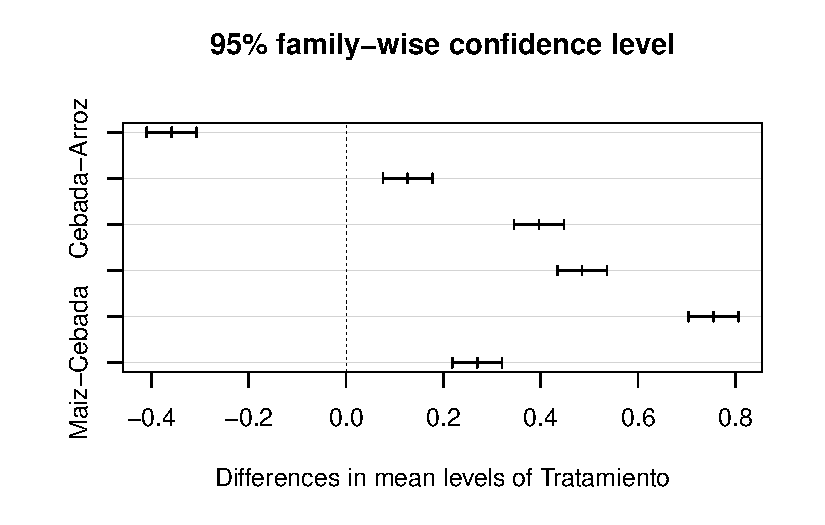
\includegraphics[keepaspectratio]{Chapter_02_files/figure-pdf/unnamed-chunk-11-1.pdf}}

\textbf{Interpretación:} El gráfico muestra los intervalos de confianza
del 95\,\% para las diferencias de medias entre los tratamientos,
ajustados por comparaciones múltiples (family-wise). Ninguno de los
intervalos cruza la línea vertical en cero, lo cual indica que todas las
comparaciones entre pares de tratamientos son estadísticamente
significativas. La diferencia más grande se observa entre Maíz y Avena,
mientras que la más pequeña, aunque significativa, es entre Cebada y
Arroz. Este resultado es coherente con los análisis previos (ANOVA, LSD
y Scheffé), y respalda que cada tratamiento tiene un efecto
significativamente distinto sobre la variable ``Resultado''.

\begin{Shaded}
\begin{Highlighting}[]
\FunctionTok{scheffe.test}\NormalTok{(Anova, }\StringTok{"Tratamiento"}\NormalTok{,}\AttributeTok{console=}\ConstantTok{TRUE}\NormalTok{)}
\end{Highlighting}
\end{Shaded}

\begin{verbatim}

Study: Anova ~ "Tratamiento"

Scheffe Test for Resultado 

Mean Square Error  : 0.0005953124 

Tratamiento,  means

       Resultado        std r         se      Min      Max      Q25      Q50
Arroz   8.733890 0.02192214 4 0.01219951 8.715318 8.762183 8.717232 8.729030
Avena   8.375414 0.02519485 4 0.01219951 8.341039 8.395990 8.364419 8.382314
Cebada  8.860578 0.03330518 4 0.01219951 8.822181 8.900695 8.842075 8.859719
Maiz    9.130190 0.01251613 4 0.01219951 9.113429 9.140539 9.124249 9.133395
            Q75
Arroz  8.745688
Avena  8.393309
Cebada 8.878222
Maiz   9.139335

Alpha: 0.05 ; DF Error: 12 
Critical Value of F: 3.490295 

Minimum Significant Difference: 0.05582762 

Means with the same letter are not significantly different.

       Resultado groups
Maiz    9.130190      a
Cebada  8.860578      b
Arroz   8.733890      c
Avena   8.375414      d
\end{verbatim}

\textbf{Interpretación:} A pesar de ser una prueba más conservadora, el
test de Scheffé también encontró diferencias significativas entre todos
los tratamientos. El análisis agrupó los tratamientos en distintos
niveles.Mínima diferencia significativa (Scheffé): 0.0558. Valor crítico
de F: 3.4903

\textbf{Conclusión general} Las tres pruebas aplicadas (LSD, Tukey y
Scheffé) coinciden en que todos los tratamientos difieren
significativamente entre sí. El tratamiento con mayor rendimiento fue
Maíz, seguido por Cebada, Arroz y Avena, en orden descendente. Esto
respalda la conclusión de que el tipo de tratamiento influye de manera
significativa sobre la variable respuesta.

\subsubsection{2.2.2 Diseño de bloques completamente al azar
OK}\label{diseuxf1o-de-bloques-completamente-al-azar-ok}

\subsubsection{2.2.3 Diseño longitudinal (ANOVA de medidas repetidas)
OK}\label{diseuxf1o-longitudinal-anova-de-medidas-repetidas-ok}

\bookmarksetup{startatroot}

\chapter{Parte III: Uso de Inteligencia Artificial para la simulación de
datos}\label{parte-iii-uso-de-inteligencia-artificial-para-la-simulaciuxf3n-de-datos}

\section{Uso de Inteligencia Artificial para la simulación de
datos.}\label{uso-de-inteligencia-artificial-para-la-simulaciuxf3n-de-datos.}

\subsection{}\label{section}

\bookmarksetup{startatroot}

\chapter*{References}\label{references}
\addcontentsline{toc}{chapter}{References}

\markboth{References}{References}

\phantomsection\label{refs}
\begin{CSLReferences}{1}{0}
\bibitem[\citeproctext]{ref-Wickham2017R}
Grolemund, Garrett, and Hadley Wickham. 2017. \emph{R for Data Science}.
O'Reilly Media.

\bibitem[\citeproctext]{ref-Peng2011}
Peng, Roger D. 2011. {``Reproducible Research in Computational
Science.''} \emph{Science} 334 (6060): 1226--27.
\url{https://doi.org/10.1126/science.1213847}.

\bibitem[\citeproctext]{ref-Rcore2021}
R Core Team. 2021. \emph{R: A Language and Environment for Statistical
Computing}. Vienna, Austria: R Foundation for Statistical Computing.
\url{https://www.R-project.org/}.

\bibitem[\citeproctext]{ref-Reeder2021}
Reeder, Janina, Mo Huang, Joshua S Kaminker, and Joseph N Paulson. 2021.
{``{MicrobiomeExplorer: an R package for the analysis and visualization
of microbial communities.}''} \emph{Bioinformatics (Oxford, England)} 37
(9): 1317--18. \url{https://doi.org/10.1093/bioinformatics/btaa838}.

\bibitem[\citeproctext]{ref-wickham2016a}
Wickham, Hadley. 2016. \emph{Ggplot2}. Springer International
Publishing. \url{https://doi.org/10.1007/978-3-319-24277-4}.

\bibitem[\citeproctext]{ref-wickham2015}
Wickham, Hadley, and Jennifer Bryan. 2015. {``Readxl: Read Excel
Files.''} The R Foundation.
\url{https://doi.org/10.32614/cran.package.readxl}.

\bibitem[\citeproctext]{ref-Zhou2012}
Zhou, Bin, Jun Feng Xiao, Leepika Tuli, and Habtom W Ressom. 2012.
{``{LC-MS-based metabolomics.}''} \emph{Molecular bioSystems} 8 (2):
470--81. \url{https://doi.org/10.1039/c1mb05350g}.

\end{CSLReferences}




\end{document}
